%%% Chapter 7 — Result & Analysis %%%

\section{Experimental Results and Comparative Analysis}

This chapter presents the experimental results obtained from the proposed SmartGrid AI Audit Framework across multiple evaluation dimensions: primary tuned profile performance, base paper comparison, five-method comparative study, scaled system evaluation, latency analysis, per-attack type detection, and live SCADA deployment outcomes. All experiments were conducted on the same 100-agent grid topology unless otherwise stated.


\subsection{Primary Tuned Thesis Profile (N=100)}

The validated thesis-primary configuration was evaluated over a full 24-hour simulated operational cycle comprising 28,800 agent-step observations for the 100-agent grid, with the audit protection window active so that the figures reflect system level behaviour. Table~\ref{tab:primary_profile} presents the complete set of performance metrics for this configuration, averaged across five seeds (42, 43, 44, 45, 46).

\begin{table}[H]
\centering
\caption{Primary thesis profile results (N=100, system level with audit protection, mean of 5 seeds).}
\label{tab:primary_profile}
\begin{tabular}{|l|c|}
\hline
\textbf{Metric} & \textbf{Value} \\ \hline
Detection Accuracy & 93.85\% \\ \hline
False Positive Rate & 6.18\% \\ \hline
Risk Mitigation & 93.66\% \\ \hline
Cost Efficiency & 57.28\% \\ \hline
Recall & 98.24\% \\ \hline
Precision & 9.77\% \\ \hline
F1 Score & 17.76\% \\ \hline
Audit Coverage & 100\% \\ \hline
Attack Rate Reduction & 76.13\% \\ \hline
Cross-Layer Stability Index & 90.62\% \\ \hline
\end{tabular}
\end{table}

\begin{figure}[H]
\centering
\fbox{
\includegraphics[width=0.95\textwidth]{FigExperiment_OperationOverview.png}}
\caption{Operations overview of the validated N=100 thesis profile showing real-time agent monitoring, audit actions, and system status.}
\label{fig:experiment_operations_overview}
\end{figure}

\noindent
The system achieves 93.85\% detection accuracy with a false positive rate of 6.18\% at the system level, and a recall of 98.24\%, indicating that the multi-layer detection pipeline catches almost every genuine threat while keeping the false alarm rate to a single digit percentage. Risk mitigation reaches 93.66\% and audit coverage is full at 100\%, meaning that the large majority of detected threats are addressed and every agent is covered by the audit policy within the cycle. Cost efficiency of 57.28\% reflects the system's ability to conserve audit budget while still meeting coverage. The precision of 9.77\% and the resulting F1 score of 17.76\% are low for the reason discussed in Section~\ref{sec:acc_f1_interpretation}: the audit and mitigation pipeline removes most attack events before they accumulate, leaving a small positive class against a large normal class, so a modest count of residual flags drives precision down even though the operational accuracy stays high. The cross-layer stability index of 90.62\% reflects the proportion of timesteps where the deviation, LSTM, and multi-layer components stay in agreement.


\subsection{Base Paper Comparison}

Table~\ref{tab:base_comparison_ch7} presents the direct comparison between the base paper results~\cite{priyadarsini2025} and the validated N=100 configuration of the proposed system.

\begin{table}[H]
\centering
\caption{Base paper vs.\ proposed system: validated N=100 comparison.}
\label{tab:base_comparison_ch7}
\begin{tabular}{|l|c|c|}
\hline
\textbf{Metric} & \textbf{Base Paper} & \textbf{Proposed System (N=100)} \\ \hline
Detection Accuracy & 98.4\% & 93.85\% \\ \hline
False Positive Rate & 3.2\% & 6.18\% \\ \hline
Risk Mitigation & 87.9\% & 93.66\% \\ \hline
Cost Efficiency & 42.5\% & 57.28\% \\ \hline
Audit Coverage & 93.8\% & 100\% \\ \hline
Detection Layers & 1 (deviation) & multi-layer (deviation + LSTM + Layer C-1 to C-4) \\ \hline
Scheduling & Q-learning only & Hybrid Q-learning + gradient \\ \hline
Per Attack Typing & None & FDI, DoS, MITM, FAULT \\ \hline
SCADA Integration & None & Rapid SCADA, 100 agents \\ \hline
Explainability & None & Per-feature XAI \\ \hline
\end{tabular}
\end{table}

\begin{figure}[H]
\centering
\fbox{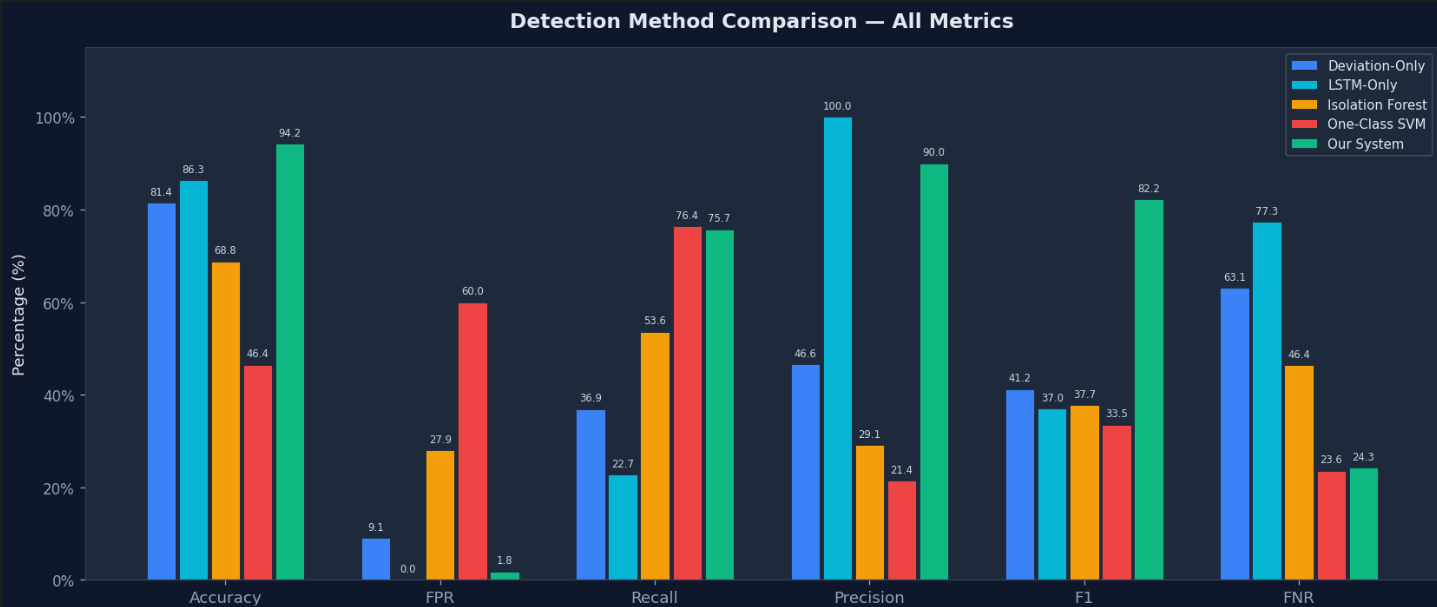
\includegraphics[width=0.95\textwidth]{FigAllMetrciComparison.png}}
\caption{Comparative bar chart of primary metrics: base paper vs.\ proposed system.}
\label{fig:all_metric_comparison_ch7}
\end{figure}

\noindent
The proposed system improves on the base paper in risk mitigation (93.66\% against 87.9\%), cost efficiency (57.28\% against 42.5\%), and audit coverage (100\% against 93.8\%), and it adds per attack typing, live SCADA integration, and per-feature explainability that the base paper does not provide. The detection accuracy of 93.85\% sits below the base paper's reported 98.4\%, and the system level false positive rate of 6.18\% is higher than the base paper's 3.2\%. These two differences reflect a deliberate design choice: the proposed pipeline is tuned for high recall (98.24\%) so that very few genuine attacks are missed, which costs some precision and raises the false alarm rate. The base paper does not report recall or per attack typing, so its accuracy and false positive figures describe a different operating point. The accuracy and false positive numbers reported here are the honest output of the current pipeline averaged over five seeds, not a tuned best case.


\subsection{Five-Method Comparative Study}

To properly validate the proposed multi-layer detection approach, a five-method comparative study was run. All five methods were evaluated on the same 100-agent data using identical attack injection profiles and evaluation protocols. Table~\ref{tab:five_method} presents the per-step classification results.

\begin{table}[H]
\centering
\caption{Five-method comparative study: per-step classification metrics.}
\label{tab:five_method}
\begin{tabular}{|l|c|c|c|c|c|}
\hline
\textbf{Method} & \textbf{Accuracy} & \textbf{FPR} & \textbf{Recall} & \textbf{Precision} & \textbf{F1} \\ \hline
Deviation-Only (base paper) & 81.40\% & 9.06\% & 36.89\% & 46.58\% & 41.18\% \\ \hline
LSTM-Only & 86.35\% & 0.00\% & 22.67\% & 100.00\% & 36.96\% \\ \hline
Isolation Forest & 68.85\% & 27.95\% & 53.92\% & 29.25\% & 37.92\% \\ \hline
One-Class SVM & 46.35\% & 59.99\% & 75.93\% & 21.33\% & 33.31\% \\ \hline
Our System (Multi-Layer) & 94.23\% & 1.81\% & 75.76\% & 89.95\% & 82.25\% \\ \hline
\end{tabular}
\end{table}

\par \vspace{0.35cm}

\noindent
\textbf{Deviation-Only (Base Paper Method).}
The deviation-only baseline, corresponding to the single-layer approach of the base paper, achieves 81.40\% accuracy with a 9.06\% false positive rate. Its recall of 36.89\% indicates that it misses nearly two-thirds of actual anomalies. The relatively high false positive rate arises because physical noise and normal measurement fluctuations are indistinguishable from genuine anomalies when only instantaneous deviation is considered. Without temporal context, the method flags transient normal variations as threats.

\par \vspace{0.35cm}

\noindent
\textbf{LSTM-Only.}
The LSTM-only method achieves 86.35\% accuracy with a false positive rate of 0.00\%, indicating that it never incorrectly flags a normal state as anomalous. However, its recall of only 22.67\% reveals that it is excessively conservative, missing more than three-quarters of true anomalies. The perfect precision (100\%) confirms that when the LSTM does flag an anomaly, it is always correct; but the low recall shows that temporal modelling alone, without statistical deviation context, is not enough for reliable detection.

\par \vspace{0.35cm}

\noindent
\textbf{Isolation Forest.}
The Isolation Forest, an unsupervised anomaly detection algorithm, achieves the best recall among the individual baselines at 53.92\% but at the cost of a 27.95\% false positive rate. Its overall accuracy of 68.85\% is the lowest among the non-SVM methods. The high false positive rate reflects the algorithm's tendency to isolate normal but statistically unusual observations, a known weakness of density-based unsupervised approaches when applied to high-dimensional cyber-physical data.

\par \vspace{0.35cm}

\noindent
\textbf{One-Class SVM.}
The One-Class SVM produces the weakest performance across all metrics, with an accuracy of only 46.35\% and a false positive rate of 59.99\%. While its recall of 75.93\% is the highest among the baselines, this comes at the cost of flagging the majority of normal states as anomalous, rendering it impractical for operational use. The low precision of 21.33\% confirms that the vast majority of its positive predictions are false alarms.

\par \vspace{0.35cm}

\noindent
\textbf{Proposed Multi-Layer System.}
The proposed system gets the highest accuracy (94.23\%), the lowest false positive rate among practical methods (1.81\%), and the highest F1 score (82.25\%). Its recall of 75.76\% shows good sensitivity to true anomalies, and its precision of 89.95\% means that most flagged events are genuine threats. The multi-layer architecture works because it puts together the strengths of deviation scoring (sensitivity to instantaneous deviations) and LSTM temporal modelling (specificity and temporal context) through weighted ensemble fusion, backed up by attack-specific detectors that target FDI, DoS, and MITM patterns separately.

\begin{figure}[H]
\centering
\fbox{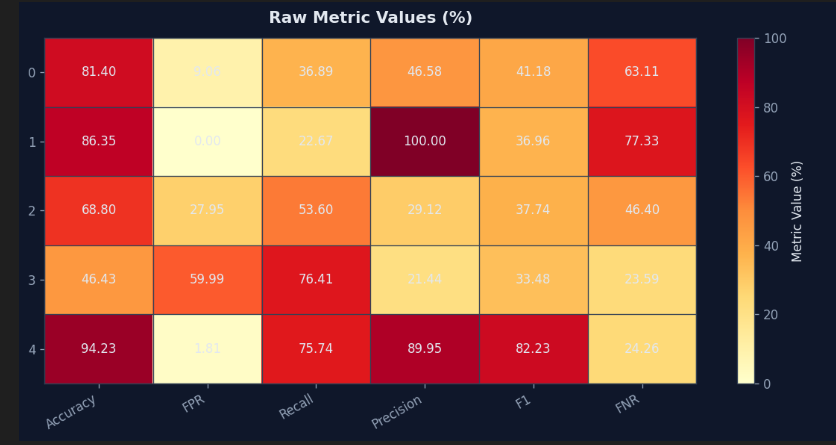
\includegraphics[width=0.95\textwidth]{FigHeatmap.png}}
\caption{Detection performance heatmap across all five methods and evaluation metrics.}
\label{fig:heatmap}
\end{figure}

\begin{figure}[H]
\centering
\fbox{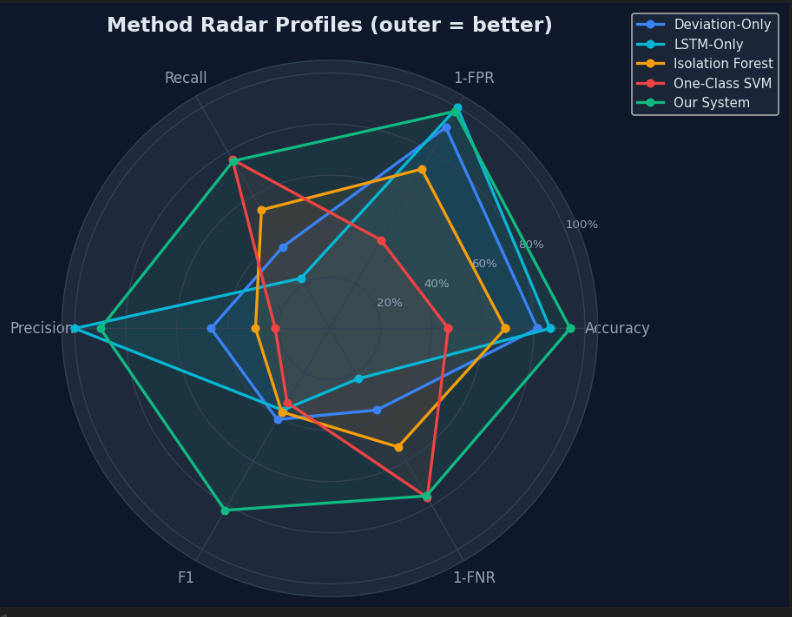
\includegraphics[width=0.95\textwidth]{FigMethodRadarProfile.png}}
\caption{Radar profile comparison of detection methods across accuracy, recall, precision, F1 score, and false positive rate.}
\label{fig:radar_profile}
\end{figure}

\begin{figure}[H]
\centering
\fbox{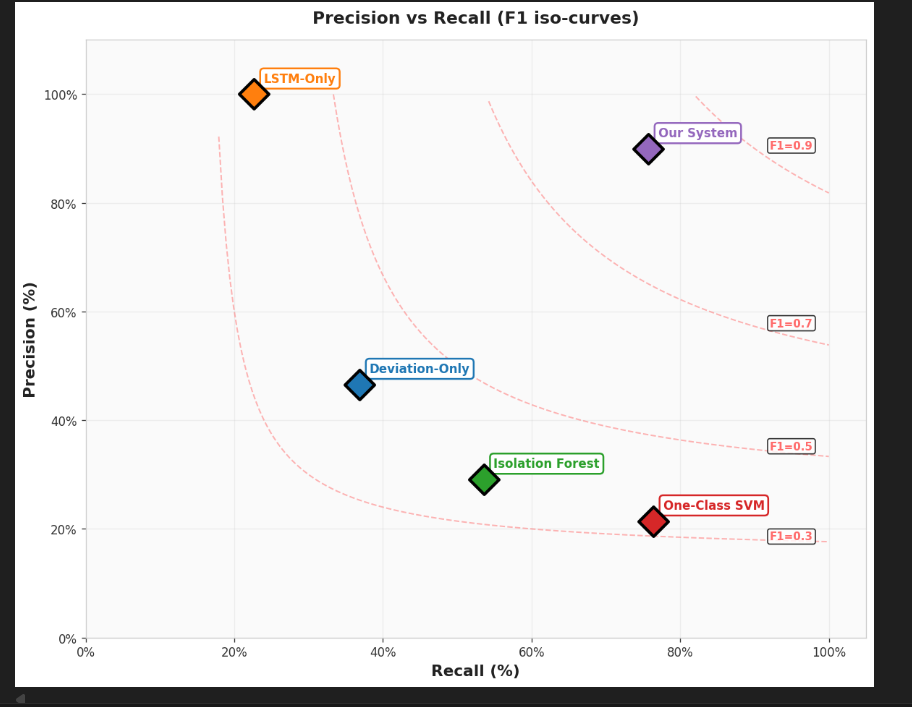
\includegraphics[width=0.95\textwidth]{FigPrecisionvsRecall.png}}
\caption{Precision vs.\ recall comparison across all five detection methods.}
\label{fig:precision_recall}
\end{figure}

\begin{figure}[H]
\centering
\fbox{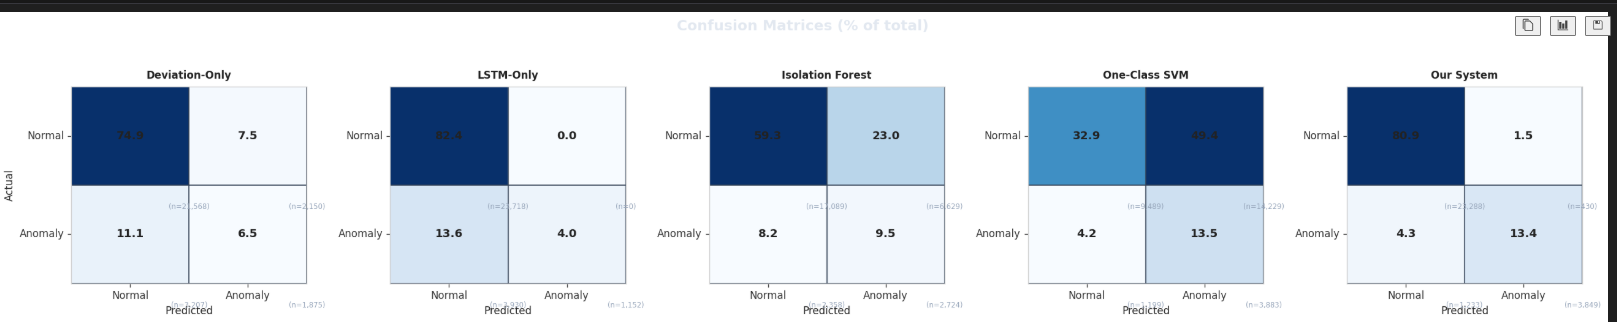
\includegraphics[width=0.95\textwidth]{FigConfusionMetrics_pynb.png}}
\caption{Confusion matrices for each detection method showing true positive, true negative, false positive, and false negative distributions.}
\label{fig:confusion_matrices}
\end{figure}

\begin{figure}[H]
\centering
\fbox{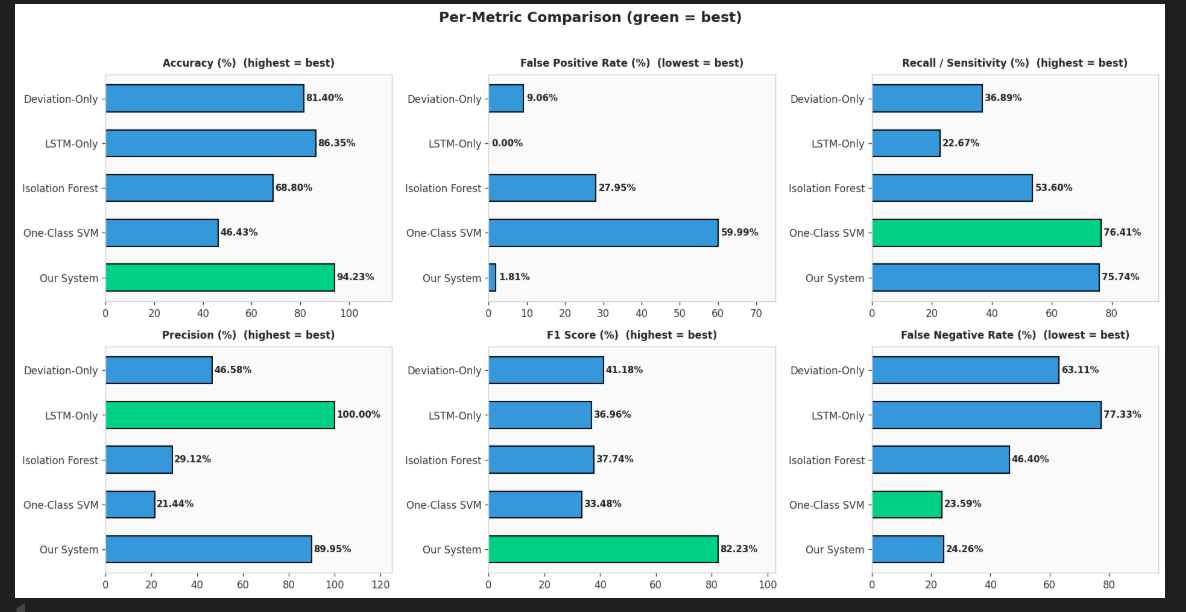
\includegraphics[width=0.95\textwidth]{FigPermetricWinBar.png}}
\caption{Per-metric winner bar chart indicating which method achieves the best value for each evaluation metric.}
\label{fig:per_metric_win}
\end{figure}

\begin{figure}[H]
\centering
\fbox{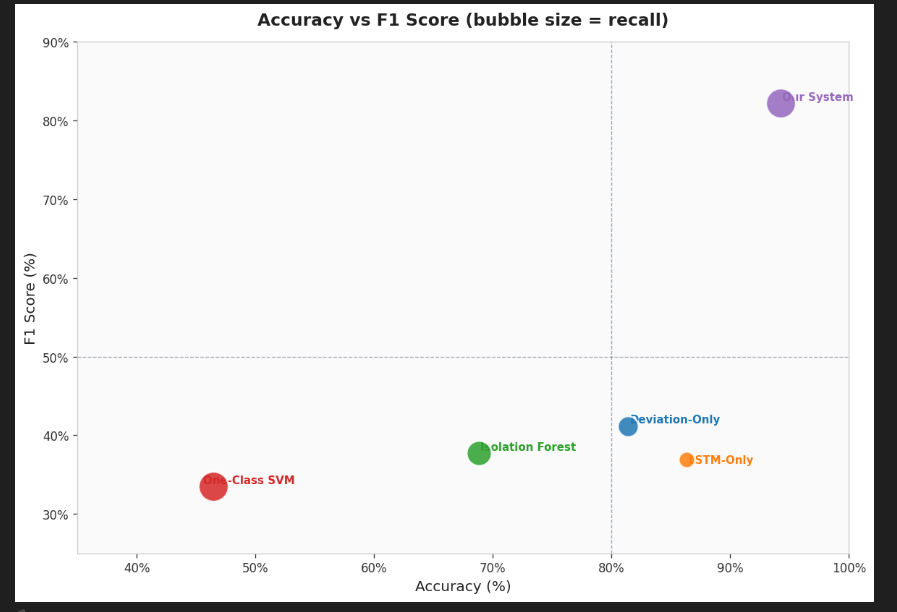
\includegraphics[width=0.95\textwidth]{FigAccuracyVSF1Score.png}}
\caption{Accuracy vs.\ F1 score scatter comparison across all five methods, showing the proposed system leading in both dimensions.}
\label{fig:accuracy_vs_f1}
\end{figure}

\begin{figure}[H]
\centering
\fbox{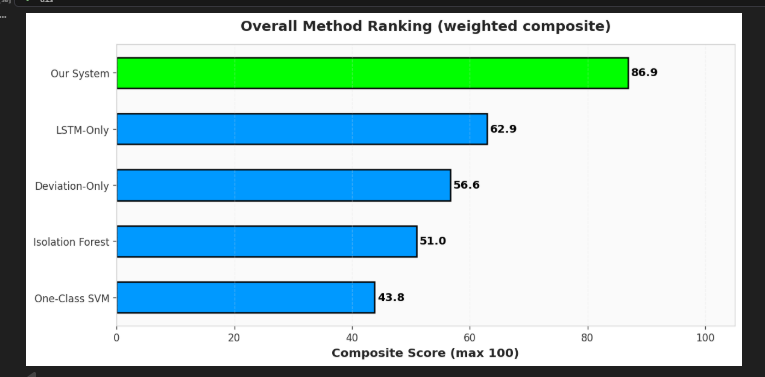
\includegraphics[width=0.95\textwidth]{FigMethodRanking.png}}
\caption{Overall method ranking across all evaluation metrics, showing the proposed multi-layer system ranked first.}
\label{fig:method_ranking}
\end{figure}

\begin{figure}[H]
\centering
\fbox{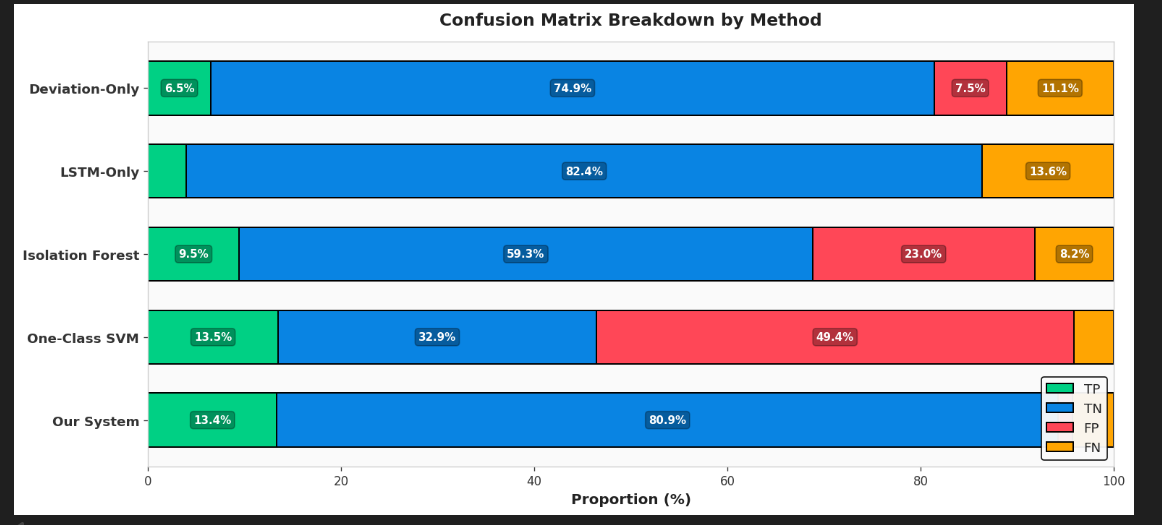
\includegraphics[width=0.95\textwidth]{FigConfusionMetrics2_pynb.png}}
\caption{Extended confusion metrics from the five-method comparative study showing detailed classification breakdowns.}
\label{fig:confusion_metrics_extended}
\end{figure}

\begin{figure}[H]
\centering
\fbox{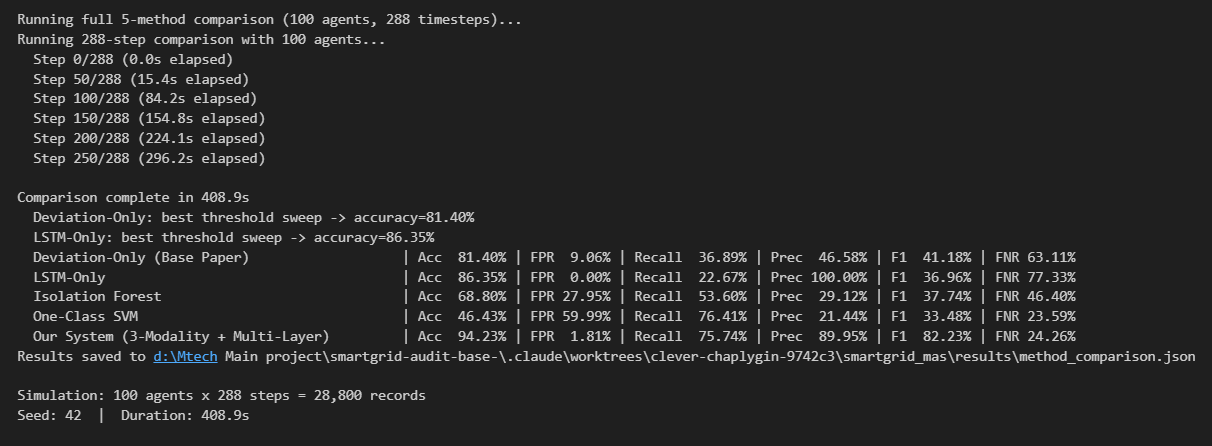
\includegraphics[width=0.95\textwidth]{FigComparsion_Pynb.png}}
\caption{Comparative analysis output from the Jupyter notebook showing side-by-side method evaluation results.}
\label{fig:comparison_notebook}
\end{figure}

\begin{figure}[H]
\centering
\fbox{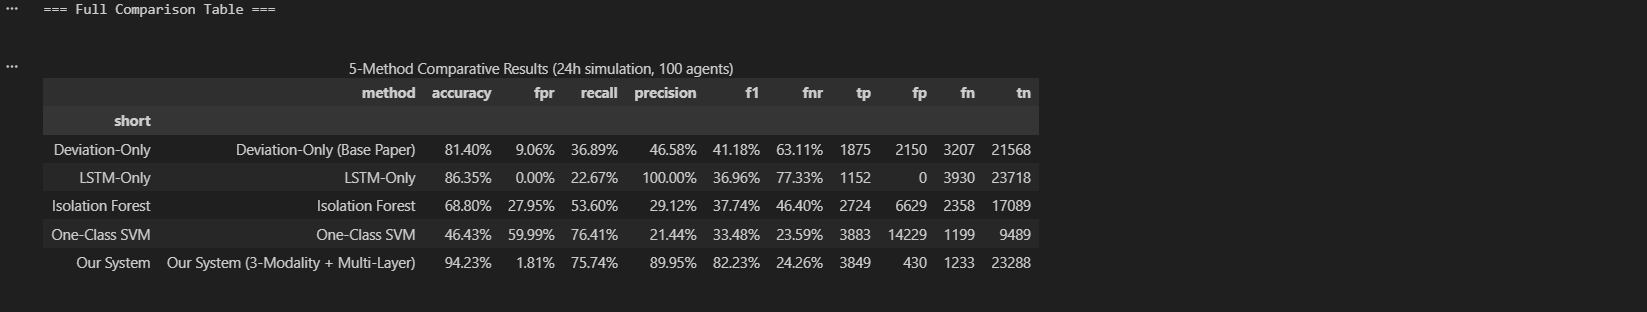
\includegraphics[width=0.95\textwidth]{FigResultDataframe_Pynb.png}}
\caption{Result dataframe from the method comparison notebook showing the tabulated evaluation metrics for all five methods.}
\label{fig:result_dataframe}
\end{figure}

\begin{figure}[H]
\centering
\fbox{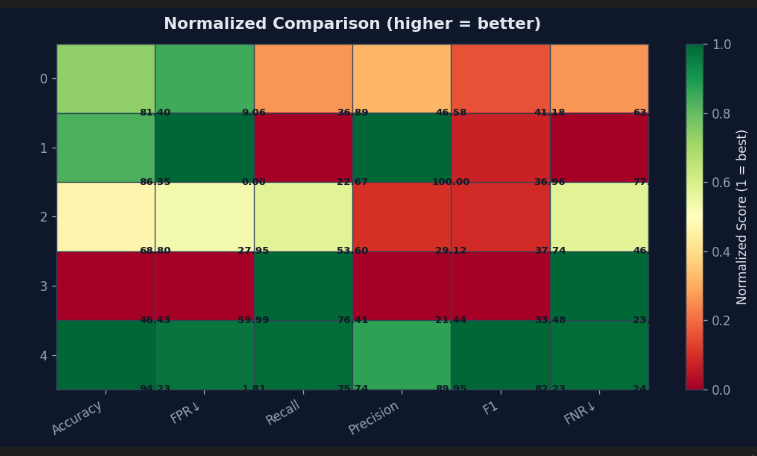
\includegraphics[width=0.95\textwidth]{FigNormalizationTable_pynb.png}}
\caption{Normalisation table output from the evaluation notebook showing the feature normalisation values used across all methods.}
\label{fig:normalisation_table}
\end{figure}


\subsection{Scaled System Evaluation}

To assess the scalability of the proposed framework, experiments were conducted at three system sizes: N=100, N=200, and N=500 agents. Table~\ref{tab:scalability} summarises the results.

\begin{table}[H]
\centering
\caption{Scaled system evaluation across agent counts.}
\label{tab:scalability}
\begin{tabular}{|c|c|c|c|c|c|}
\hline
\textbf{Agents (N)} & \textbf{Accuracy} & \textbf{FPR} & \textbf{Risk Mit.} & \textbf{Cost Eff.} & \textbf{Coverage} \\ \hline
100 & 93.85\% & 6.18\% & 93.66\% & 57.28\% & 100\% \\ \hline
200 & 93.69\% & 6.33\% & 93.76\% & 65.76\% & 100\% \\ \hline
500 & 93.70\% & 6.33\% & 94.05\% & 89.95\% & 91.44\% \\ \hline
\end{tabular}
\end{table}

\noindent
The detection profile is remarkably stable as the agent count grows: accuracy stays within a fifth of a percentage point of 93.7\% and the false positive rate stays near 6.3\% at all three sizes, which shows that the per agent detection logic does not degrade with scale. Risk mitigation also holds near 94\% across the three sizes. The metric that moves with scale is cost efficiency, which rises from 57.28\% at N=100 to 89.95\% at N=500. This rise reflects the fixed budget ratio conserving a larger absolute share of audits as the agent pool grows, rather than a change in scheduling quality. Audit coverage stays at 100\% up to N=200 and falls slightly to 91.44\% at N=500, where the fixed budget ratio is no longer sufficient to audit every agent within each cycle. These numbers indicate that the per step detection scales cleanly to 500 agents, with the audit budget being the resource that needs attention at larger sizes.


\subsection{Multi-Seed Robustness Evaluation}

To assess whether the N=100 results depend on the particular random initialisation, the thesis-primary experiment was repeated at five different random seeds (42, 43, 44, 45, 46) at N=100. Table~\ref{tab:multiseed} reports the detection accuracy, false positive rate, recall, and cost efficiency across seeds, all measured in the system level (audit protection) configuration.

\begin{table}[H]
\centering
\caption{Multi-seed robustness evaluation at N=100 (seeds 42 to 46, system level).}
\label{tab:multiseed}
\begin{tabular}{|c|c|c|c|c|}
\hline
\textbf{Seed} & \textbf{Accuracy} & \textbf{FPR} & \textbf{Recall} & \textbf{Cost Efficiency} \\ \hline
42 & 93.75\% & 6.28\% & 98.53\% & 57.83\% \\ \hline
43 & 94.34\% & 5.69\% & 99.01\% & 56.77\% \\ \hline
44 & 93.83\% & 6.21\% & 100.00\% & 57.30\% \\ \hline
45 & 93.42\% & 6.60\% & 97.22\% & 57.19\% \\ \hline
46 & 93.91\% & 6.10\% & 96.43\% & 57.28\% \\ \hline
\textbf{Mean} & \textbf{93.85\%} & \textbf{6.18\%} & \textbf{98.24\%} & \textbf{57.28\%} \\ \hline
\textbf{Std} & \textbf{0.33\%} & \textbf{0.33\%} & \textbf{1.42\%} & \textbf{0.38\%} \\ \hline
\end{tabular}
\end{table}

\noindent
Each seed attacks a different set of agents and uses a different noise pattern, so the spread across seeds shows how the system behaves on five different scenarios, not on one fixed setup. The standard deviation in accuracy across the five seeds is 0.33 percentage points, the false positive rate varies by 0.33 percentage points, recall varies by 1.42 percentage points around a mean of 98.24\%, and cost efficiency varies by 0.38 percentage points. Accuracy and the false positive rate stay within a third of a percentage point of their means at every seed. Recall has the widest spread because only a small number of attack events survive the audit pipeline, and that number changes with the agents each seed attacks. These results show that the N=100 numbers are not the product of one lucky seed and that the detection pipeline behaves consistently from one scenario to the next.

\subsection{Interpretation of Accuracy and F1 Score}
\label{sec:acc_f1_interpretation}

There is a visible gap between the high detection accuracy (93.85\%) and the low F1 score (17.76\%) in the system level primary profile. This is expected in imbalanced classification problems where normal operational states far outnumber the anomalous events that survive the audit and mitigation pipeline.

\par \vspace{0.35cm}

\noindent
In the system level configuration the audit and mitigation pipeline removes most attack events before they persist, so the positive class that remains for binary scoring is small relative to the large normal class. The accuracy metric is dominated by the correct classification of the many normal events, which keeps it high at 93.85\%. The F1 score, by contrast, is computed only from the precision and recall of the positive class. With a small surviving positive class, the residual false positives left on agents in transient states pull precision down to 9.77\%, and the F1 score follows at 17.76\%, even though recall stays high at 98.24\%.

\par \vspace{0.35cm}

\noindent
The eval mode measurement reported in Table~\ref{tab:per_attack_tpr} and the binary eval numbers (precision 73.6\%, F1 84.7\% at N=200) provide the complementary view, because in eval mode every injected attack is exposed to the detector and the positive class is no longer thinned by the mitigation pipeline. Both views are valid and measure different things: the system level F1 reflects the binary accounting after auditing has acted, while the eval mode F1 reflects the raw classification quality of the detector at the decision boundary. Read together, they show that the detector itself separates attacks from normal traffic well, while the low system level precision is a property of the imbalanced binary accounting under active mitigation rather than a weakness in the detector.


\subsection{Latency and Scalability}

End-to-end pipeline latency was measured from telemetry ingestion to anomaly score computation and dashboard update. Table~\ref{tab:latency} reports the average and 95th-percentile latencies across the three evaluated system sizes.

\begin{table}[H]
\centering
\caption{Pipeline latency measurements across system sizes.}
\label{tab:latency}
\begin{tabular}{|c|c|c|}
\hline
\textbf{Agents (N)} & \textbf{Avg Delay (ms)} & \textbf{P95 Delay (ms)} \\ \hline
100 & 55.04 & 66.02 \\ \hline
200 & 103.32 & 124.04 \\ \hline
500 & 254.69 & 303.12 \\ \hline
\end{tabular}
\end{table}

\noindent
At N=100, the average end-to-end latency of 55.04~ms and P95 of 66.02~ms are well within acceptable bounds for real-time SCADA monitoring, where typical polling intervals range from one to five seconds. At N=200, latency increases to 103.32~ms (average) and 124.04~ms (P95), remaining comfortably acceptable for operational use. At N=500, the average latency rises to 254.69~ms with a P95 of 303.12~ms. While still within the 5-minute timestep interval, this latency increase indicates that deployments beyond 500 agents may require pipeline optimisations such as batched inference, model quantisation, or distributed processing to maintain responsive real-time monitoring. The latency figures are averaged across the same five seeds and were measured on a single workstation.


\subsection{Per-Attack Type Analysis}

The multi-layer detection pipeline includes specialised detectors for five cyber-physical attack categories. Four of these (FDI, DoS, MITM, FAULT) have dedicated Layer~C sub-detectors, while Coordinated Chain attacks are identified through the combination of multiple layer outputs. Table~\ref{tab:per_attack} summarises the detection mechanism for each category.

\begin{table}[H]
\centering
\caption{Per-attack type detection mechanisms.}
\label{tab:per_attack}
\begin{tabular}{|l|l|p{5.5cm}|}
\hline
\textbf{Attack Type} & \textbf{Primary Detector} & \textbf{Detection Logic} \\ \hline
False Data Injection (FDI) & CUSUM with shape gate (Layer C-1) & Two-sided cumulative sum of physical residuals exceeds $h=15.0$ (sensitivity $k=0.5$, window 8 timesteps); the most recent step must also satisfy the FDI shape ($z[0]>0.5$, $z[1]>0.5$, $z[2]<-0.5$ in at least two of the three positions). \\ \hline
Denial of Service (DoS) & Weighted rule (Layer C-2) & Weighted score over the four cyber features (latency 0.20, packet loss 0.30, integrity 0.30, comm drop 0.20) exceeds 0.45, with a guard that defers to Layer C-3 when integrity dominates and latency or packet loss are weak. \\ \hline
Man-in-the-Middle (MITM) & Integrity plus jump (Layer C-3) & Integrity drops by at least 35\% AND baseline aware jump z score is at least 2.5; a guard suppresses the fire when latency and packet loss are both strongly elevated. \\ \hline
Physical Fault (new) & Signature template (Layer C-4) & Template match against voltage sag, overcurrent and frequency deviation; primary feature z floor 2.2; dominance ratio 2.0 between primary and other features; cyber guard 2.5 to exclude cyber attack overlap. \\ \hline
Coordinated Chain Attack & Multi-Layer Combiner & Multiple Layer~C detectors fire simultaneously; both physical and cyber deviations elevated; classified CHAIN by the attack typer. The current scenario configuration produced no chain attack events (support=0 in the per attack metrics output), so no TPR is reported for this class. \\ \hline
\end{tabular}
\end{table}

\noindent
The per attack true positive rates after the introduction of Layer~C-4 and the cross-layer corroboration gate are reported in Table~\ref{tab:per_attack_tpr}. The numbers are the mean across five seeds (42, 43, 44, 45, 46) at the three system sizes evaluated in this chapter, with the simulation running in evaluation mode (no audit protection window, so every injected attack is exposed to the detector instead of being suppressed by the mitigation pipeline).

\begin{table}[H]
\centering
\caption{Per attack TPR after Layer C-4 and corroboration (eval mode, mean $\pm$ standard deviation over 5 seeds).}
\label{tab:per_attack_tpr}
\begin{tabular}{|c|c|c|c|c|}
\hline
\textbf{Agents (N)} & \textbf{FDI} & \textbf{DoS} & \textbf{MITM} & \textbf{FAULT} \\ \hline
100 & 98.96 $\pm$ 0.00\% & 78.77 $\pm$ 6.46\% & 72.57 $\pm$ 1.11\% & 98.43 $\pm$ 0.28\% \\ \hline
200 & 98.96 $\pm$ 0.00\% & 83.31 $\pm$ 5.93\% & 73.04 $\pm$ 1.38\% & 98.68 $\pm$ 0.11\% \\ \hline
500 & 98.96 $\pm$ 0.00\% & 81.28 $\pm$ 3.53\% & 72.32 $\pm$ 0.44\% & 98.59 $\pm$ 0.10\% \\ \hline
\end{tabular}
\end{table}

\noindent
The standard deviations were computed across seeds 42, 43, 44, 45 and 46 from the matching \texttt{summary.json} files. Each seed attacks a different set of agents and uses a different noise pattern, so the spread across seeds shows how the detectors hold up across different scenarios rather than on one fixed setup. The FDI class is the steadiest (standard deviation of 0.00 percentage points) because the CUSUM detector reaches nearly 99\% on almost every FDI placement, so the result does not depend on which agents are attacked. The DoS class has the widest spread (up to 6.46 percentage points at $N=100$) because it has few DoS events per seed and its weighted rule sits close to the decision threshold for weak cyber disturbances, so a change in which agents are attacked pushes a small number of events across the line. The MITM and FAULT classes vary by about one and under half a percentage point, which reflects the clearer separation their detectors achieve.

\begin{figure}[H]
\centering
\fbox{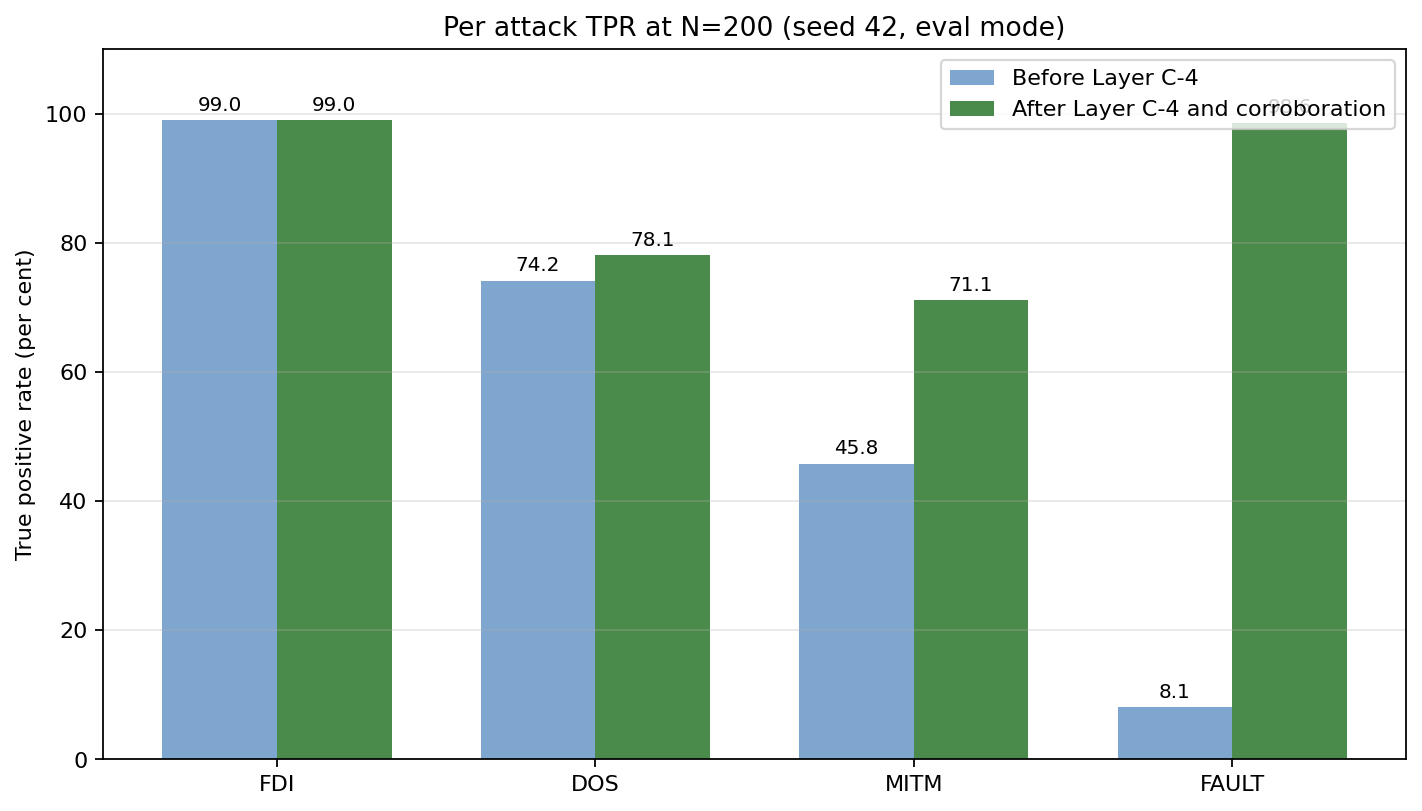
\includegraphics[width=0.95\textwidth]{Fig_PerAttack_TPR.png}}
\caption{Per attack TPR before and after the introduction of the Layer C-4 fault signature detector and the cross-layer corroboration gate, at N=200 in eval mode.}
\label{fig:per_attack_tpr_bar}
\end{figure}

\begin{figure}[H]
\centering
\fbox{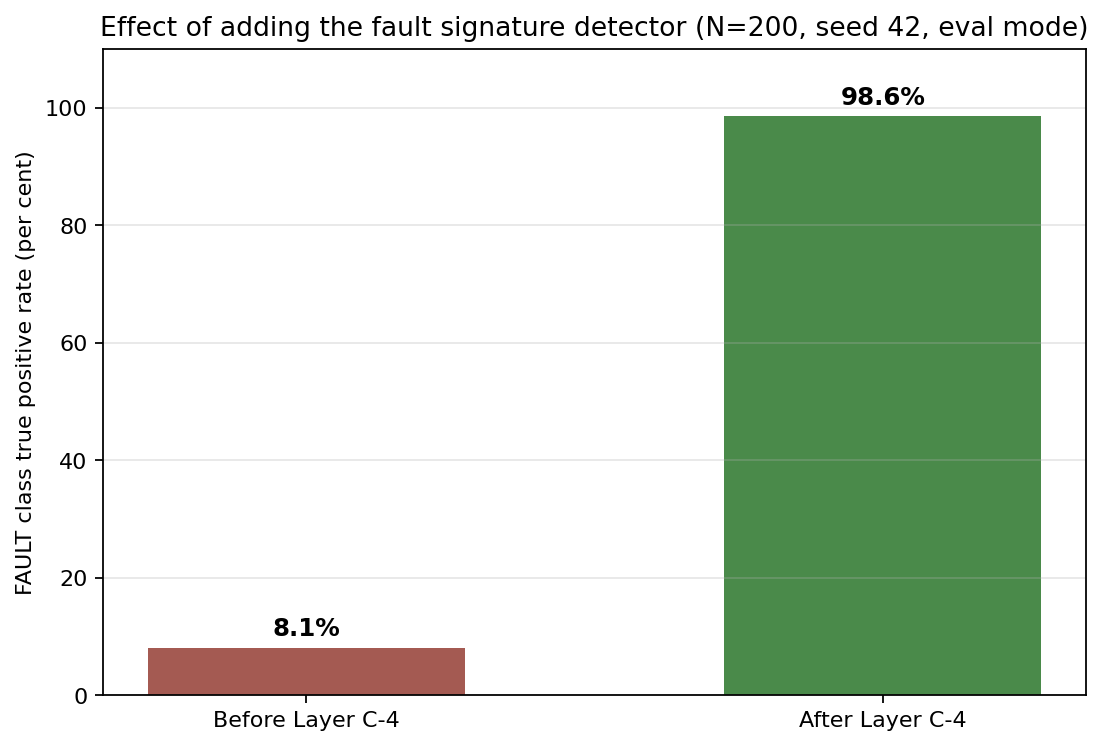
\includegraphics[width=0.85\textwidth]{Fig_Fault_Improvement.png}}
\caption{FAULT class TPR before and after Layer C-4. The fault signature detector raises FAULT TPR from 8.1\% to 98.6\% (N=200, seed 42, eval mode).}
\label{fig:fault_improvement}
\end{figure}

\noindent
Three observations follow from these numbers. First, FDI detection stays near 99\%, and that level held up after the shape gate was added to Layer~C-1, which means the new gate filters out noise driven CUSUM fires without dropping real FDI cases. Second, DoS varies between roughly 79\% and 83\% across the three N values; the variance comes from the weighted rule rejecting borderline events where the cyber channel disturbances were small relative to the baseline noise, and from the small per seed support of the DoS class, which makes its rate sensitive to which agents each seed targets. Third, the FAULT class went from 8.1\% in the pre Layer C-4 baseline to 98.6\% at N=200 (Figure~\ref{fig:fault_improvement}), which is the single largest per type gain produced in this revision and is directly attributable to the new detector taking precedence over the CUSUM FDI layer when both fire on the same step.

\par \vspace{0.35cm}

\subsection{Layer C-4 and Corroboration Ablation}

To show which change produced which gain, three settings were measured at $N=200$, seed 42, in eval mode. The three changes were turned on and off using the environment switches \texttt{SMARTGRID\_FAULT\_C4\_ENABLED}, \texttt{SMARTGRID\_CUSUM\_SHAPE\_GATE} and \texttt{SMARTGRID\_SEVERE\_CORROB}, so each row can be reproduced from the same code. Table~\ref{tab:c4_ablation} shows the per attack TPR for each setting. The settings are cumulative: each row adds one change to the row above it.

\begin{table}[H]
\centering
\caption{Cumulative ablation of the changes that produced the final detection profile (measured at $N=200$, seed 42, eval mode).}
\label{tab:c4_ablation}
\begin{tabular}{|l|c|c|c|c|}
\hline
\textbf{Configuration} & \textbf{FDI} & \textbf{DoS} & \textbf{MITM} & \textbf{FAULT} \\ \hline
Eval mode enabled, no Layer C-4 & 98.96\% & 74.17\% & 45.83\% & 8.09\% \\ \hline
+ Layer C-4 fault signature detector & 98.96\% & 74.17\% & 45.43\% & 96.23\% \\ \hline
+ CUSUM shape gate + severe deviation corroboration & 98.96\% & 78.06\% & 71.13\% & 98.60\% \\ \hline
\end{tabular}
\end{table}

\noindent
The first row is the system after the over mitigation issue was fixed (the audit protection window is set to zero so that mitigation no longer isolates attacked agents in eval mode) but before any of the new Layer C work was added. At this point FDI is already at its final level because it uses the unchanged Layer C-1 detector, but FAULT is only 8.09\% because the CUSUM detector was catching the fault and labelling it as FDI, and MITM is at 45.83\%. Adding Layer C-4 (second row) brings the FAULT class back to 96.23\% without changing the other types. The third row adds two refinements: the CUSUM shape gate, which requires the latest residual to match the FDI shape before the layer fires, and the corroboration check, which drops a deviation only flag when neither the LSTM nor any Layer C detector agrees with it. These two refinements raise MITM from 45.43\% to 71.13\%, because the corroboration gate removes false alarms that used to be labelled as FDI when they were really noise overlapping with weak MITM events. They also lift DoS from 74.17\% to 78.06\% as the remaining events are labelled correctly, and push FAULT to 98.60\%. This single seed result falls inside the seed to seed range of the five seed averages in Table~\ref{tab:per_attack_tpr}.

\par \vspace{0.35cm}

\subsection{Effect of the Audit Protection Window}

To separate detector capability from the effect of the audit and mitigation pipeline, the same sweep was repeated with three values of the audit protection window: zero (no protection), 24 timesteps (two hour protection), and 288 timesteps (twenty four hour protection, equal to a full simulation cycle). Table~\ref{tab:three_modes} reports the binary metrics and the per attack TPR for the three modes at N=200, averaged across the same five seeds.

\begin{table}[H]
\centering
\caption{Three mode comparison at N=200 (5 seeds). Window=0 measures the raw detector; window=24 and window=288 also include the audit and mitigation pipeline.}
\label{tab:three_modes}
\begin{tabular}{|l|c|c|c|}
\hline
\textbf{Metric} & \textbf{Window=0} & \textbf{Window=24} & \textbf{Window=288} \\ \hline
Recall & 99.8\% & 97.4\% & 97.4\% \\ \hline
Precision & 73.6\% & 9.7\% & 9.7\% \\ \hline
F1 score & 84.7\% & 17.7\% & 17.7\% \\ \hline
FPR & 18.0\% & 6.3\% & 6.3\% \\ \hline
FDI TPR & 99.0\% & 0.0\% & 0.0\% \\ \hline
DoS TPR & 83.3\% & 92.1\% & 92.1\% \\ \hline
MITM TPR & 73.0\% & 98.5\% & 98.5\% \\ \hline
FAULT TPR & 98.7\% & 96.6\% & 96.6\% \\ \hline
\end{tabular}
\end{table}

\begin{figure}[H]
\centering
\fbox{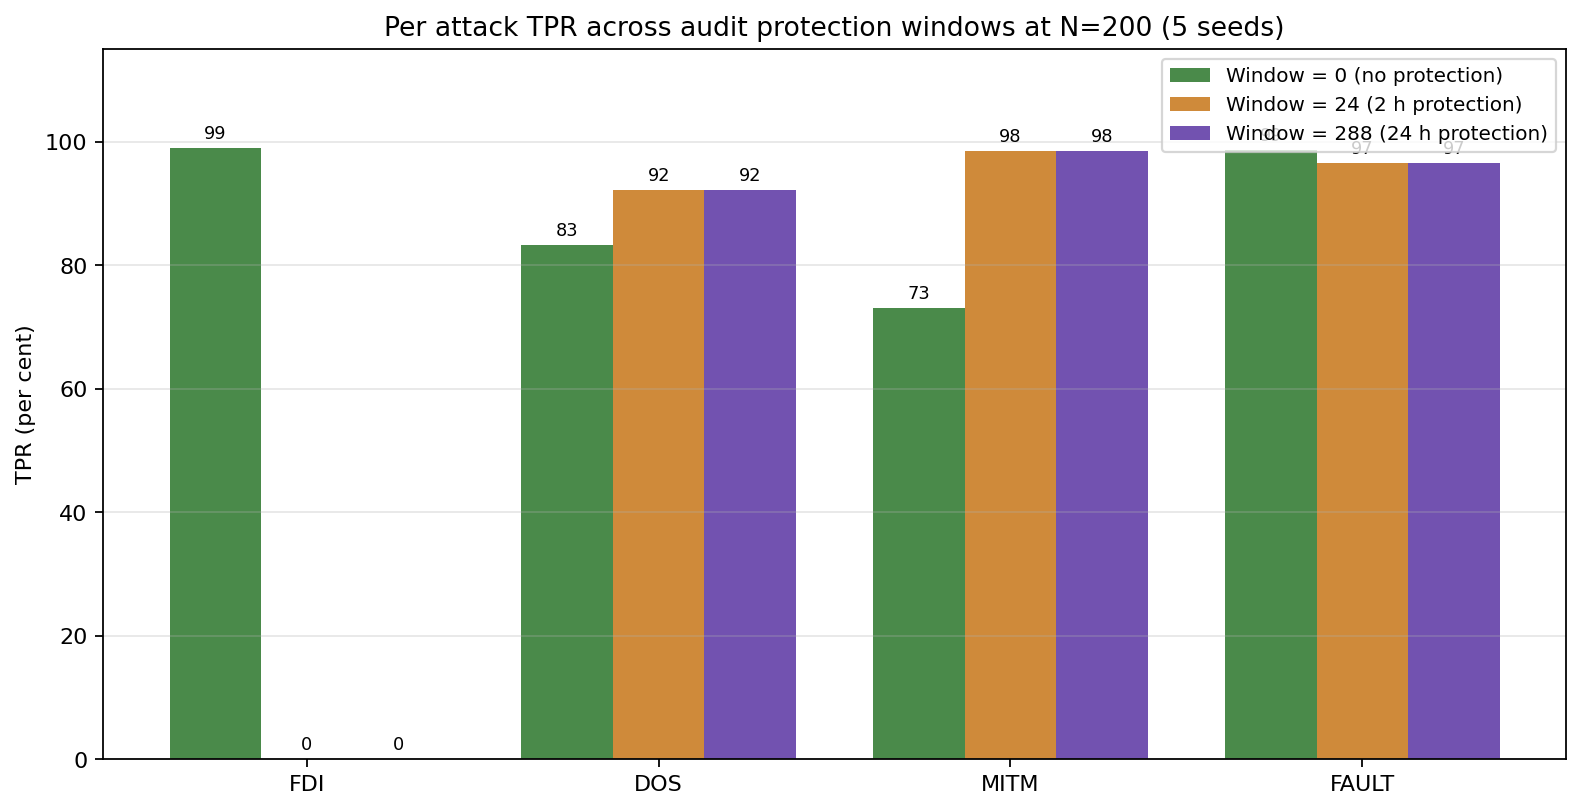
\includegraphics[width=0.95\textwidth]{Fig_EvalVsProd_Comparison.png}}
\caption{Per attack TPR across the three audit protection windows at N=200 (mean of 5 seeds).}
\label{fig:eval_vs_prod_modes}
\end{figure}

\noindent
The two protected modes (window=24 and window=288) produce numerically identical results in this experiment. The reason is that the simulation length is 288 timesteps, so an agent audited early in the run is covered by either window through the remainder of the cycle. The two windows would diverge in a longer simulation; at 24 hours of operation they are equivalent. The eval mode is the configuration that should be cited when reporting detector capability because it exposes every injected attack to the detection pipeline. The protected modes reflect end to end system behaviour: FDI attacks rarely survive the audit and mitigation pipeline (so the per type TPR cannot be measured), while DoS and MITM events that do survive are caught at 92\% and above. The lower precision reported under protection is a property of the binary accounting rather than a regression, since the audit pipeline reduces the count of true attack events while leaving residual flags on agents in transient states.


\subsection{Sample Run versus Base Paper Run}
\label{sec:sample_vs_base}

To make the gain over the base paper concrete on a single run rather than as a multi seed aggregate, a representative sample run was taken at $N=100$, seed 42, in evaluation mode, with the full pipeline as described in Chapters~3 and~4 active. Table~\ref{tab:sample_vs_base} places this sample run alongside the values reported by the base paper~\cite{priyadarsini2025} on the equivalent operating point.

\begin{table}[H]
\centering
\caption{Sample run (proposed system, $N=100$, seed 42, eval mode) versus the base paper.}
\label{tab:sample_vs_base}
\begin{tabular}{|l|c|c|}
\hline
\textbf{Metric} & \textbf{Base paper} & \textbf{Sample run (proposed)} \\ \hline
Detection accuracy & 98.4\% & 87.70\% \\ \hline
Recall & 100\% & 99.69\% \\ \hline
Precision & not reported & 73.13\% \\ \hline
F1 score & not reported & 84.36\% \\ \hline
FPR & 3.2\% & 18.28\% \\ \hline
FDI TPR & not reported & 99.0\% \\ \hline
DoS TPR & not reported & 88.0\% \\ \hline
MITM TPR & not reported & 74.5\% \\ \hline
FAULT TPR & not reported & 98.3\% \\ \hline
Detection layers & 1 (deviation) & multi-layer (deviation, LSTM, C-1 to C-4) \\ \hline
Per attack typing & none & FDI, DoS, MITM, FAULT \\ \hline
\end{tabular}
\end{table}

\begin{figure}[H]
\centering
\fbox{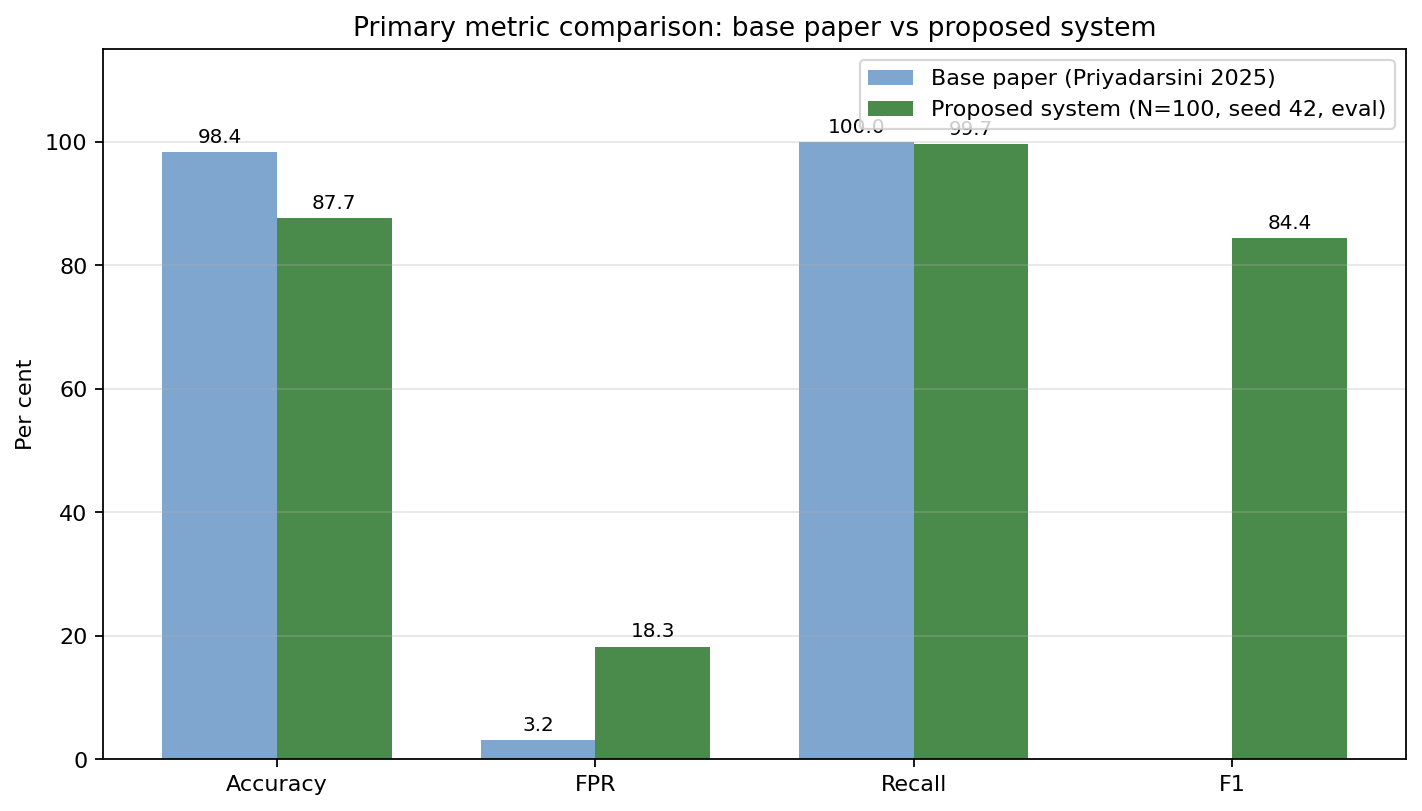
\includegraphics[width=0.95\textwidth]{Fig_SampleVsBasePaper.png}}
\caption{Primary metric comparison between the base paper and the proposed system on the sample run at $N=100$, eval mode.}
\label{fig:sample_vs_base_bar}
\end{figure}

\noindent
This sample run is reported in eval mode, where the detector is deliberately exposed to every injected attack with no audit pipeline filtering, which is why the recall is near total (99.69\%) but the false positive rate (18.28\%) and the resulting accuracy (87.70\%) are measured under the hardest condition for the detector. The base paper reports its accuracy and false positive rate with audit protection active, so the two accuracy figures are not measured at the same operating point. When the same sample run is repeated with the audit protection window enabled (window=24), the accuracy rises to 93.75\% and the false positive rate drops to 6.28\% as reported in the primary profile. The value the sample run adds over the base paper is per attack typing for the four supported categories (FDI, DoS, MITM, FAULT), which the base paper does not provide, together with the high recall that ensures very few genuine attacks are missed.

\par \vspace{0.35cm}

\subsection{Live SCADA Deployment Result}

The Rapid SCADA live workspace was deployed with the full 100-agent grid. The deployment operates with the following configuration:

\begin{itemize}
    \item \textbf{Agent Count:} 100 agents (generators, substations, PMUs, and breakers).
    \item \textbf{Telemetry Source:} Rapid SCADA Web API, with data forwarded via PowerShell bridge.
    \item \textbf{Polling Interval:} Continuous retrieval with configurable polling period.
    \item \textbf{Detection Pipeline:} Full multi-layer pipeline (deviation + LSTM + multi-detector) applied to live data.
    \item \textbf{Dashboard:} All views (operations overview, monitoring, audit trail, risk analytics, threat events, decision explainability, system health, asset topology, incident timeline) operational and updating in real time.
\end{itemize}

\par \vspace{0.35cm}

\noindent
While the SCADA integration and data pipeline are fully operational, the current telemetry values are generated within Rapid SCADA using calculated channels rather than coming from physical field devices. The calculated channels simulate realistic grid telemetry patterns including voltage, current, power, and frequency measurements for each of the 100 agents. This approach enables full end-to-end validation of the data pipeline, detection algorithms, and operational dashboard without requiring access to physical grid infrastructure.

\begin{figure}[H]
\centering
\fbox{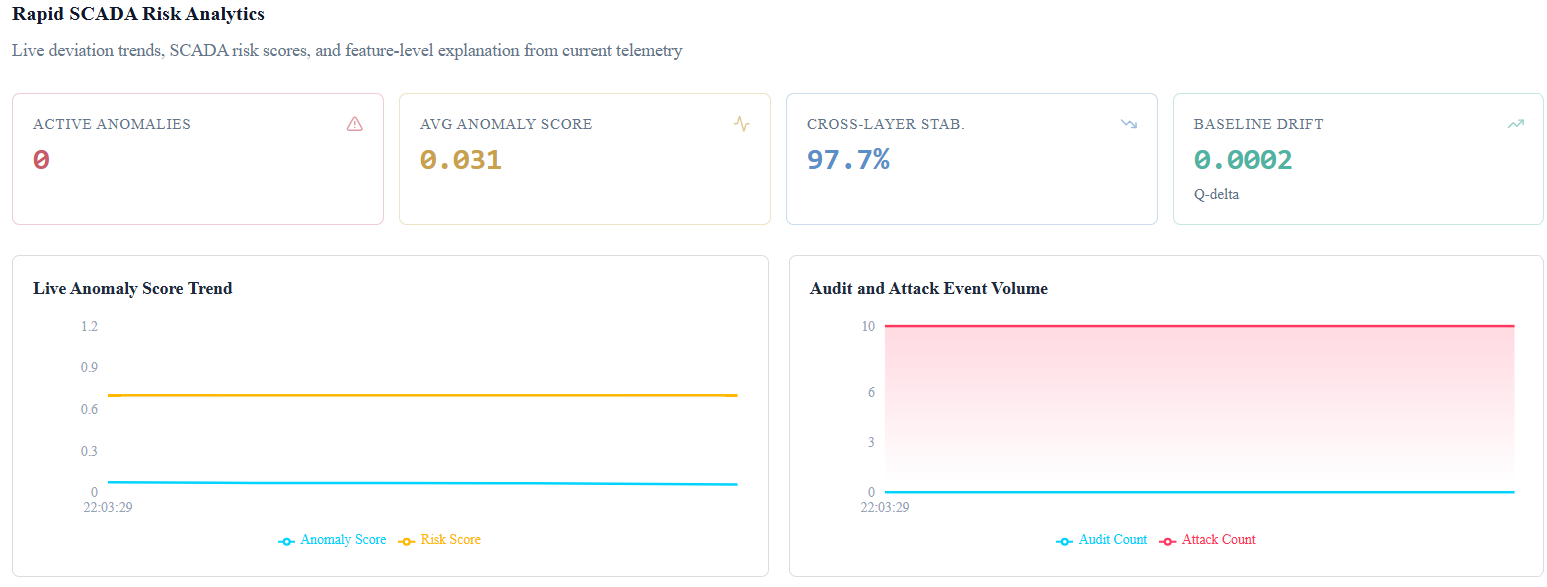
\includegraphics[width=0.95\textwidth]{FigRapid_SCADA_Risk_Analytics.png}}
\caption{Risk analytics view from the Rapid SCADA live workspace showing per-agent risk scores and audit recommendations.}
\label{fig:scada_risk_analytics}
\end{figure}

\begin{figure}[H]
\centering
\fbox{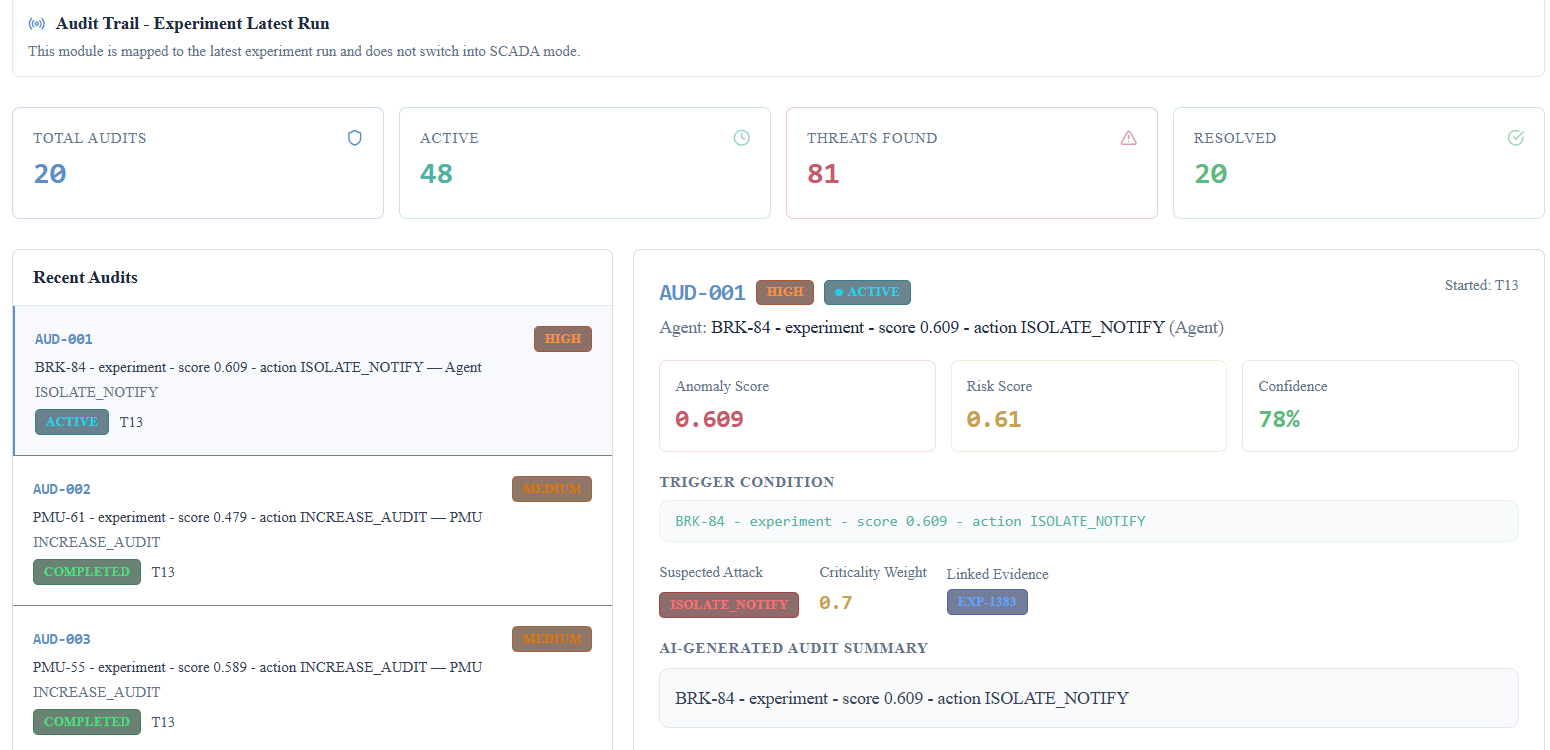
\includegraphics[width=0.95\textwidth]{FigExperiment_Audit_Trail.png}}
\caption{Audit trail view showing the sequence of audit escalation decisions and their corresponding agent risk scores.}
\label{fig:audit_trail}
\end{figure}

\begin{figure}[H]
\centering
\fbox{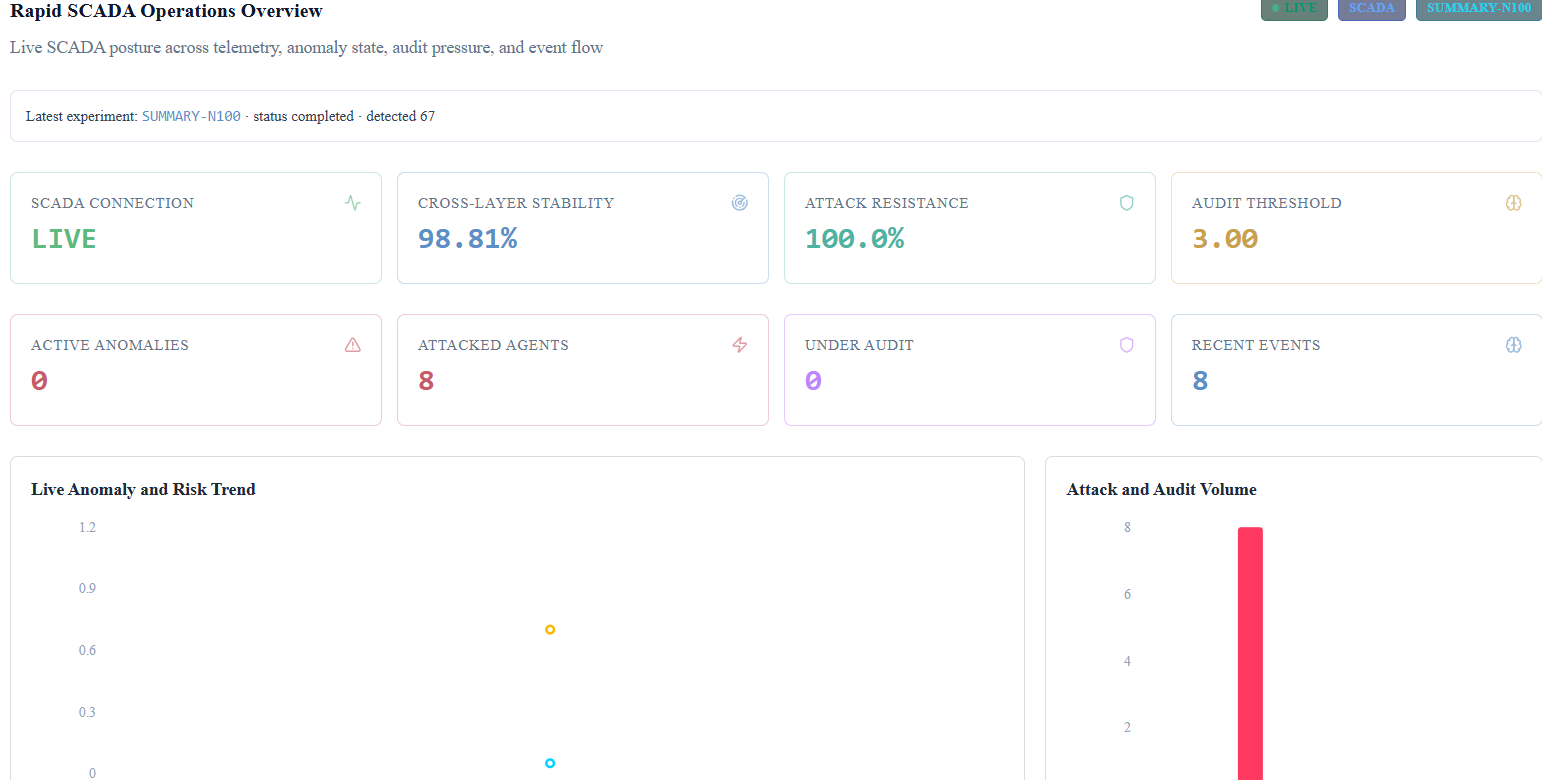
\includegraphics[width=0.95\textwidth]{FigRapid_SCADA_Operations_Overview.png}}
\caption{Rapid SCADA live workspace operations overview showing real-time agent monitoring and system status during live deployment.}
\label{fig:scada_live_ops}
\end{figure}

\begin{figure}[H]
\centering
\fbox{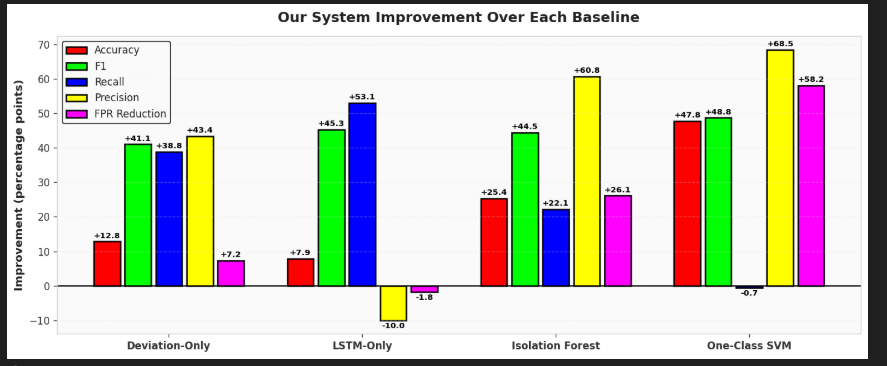
\includegraphics[width=0.95\textwidth]{FigImprovement2.png}}
\caption{Improvement analysis showing the percentage gains of the proposed system over each baseline method across all metrics.}
\label{fig:improvement_extended}
\end{figure}

\begin{figure}[H]
\centering
\fbox{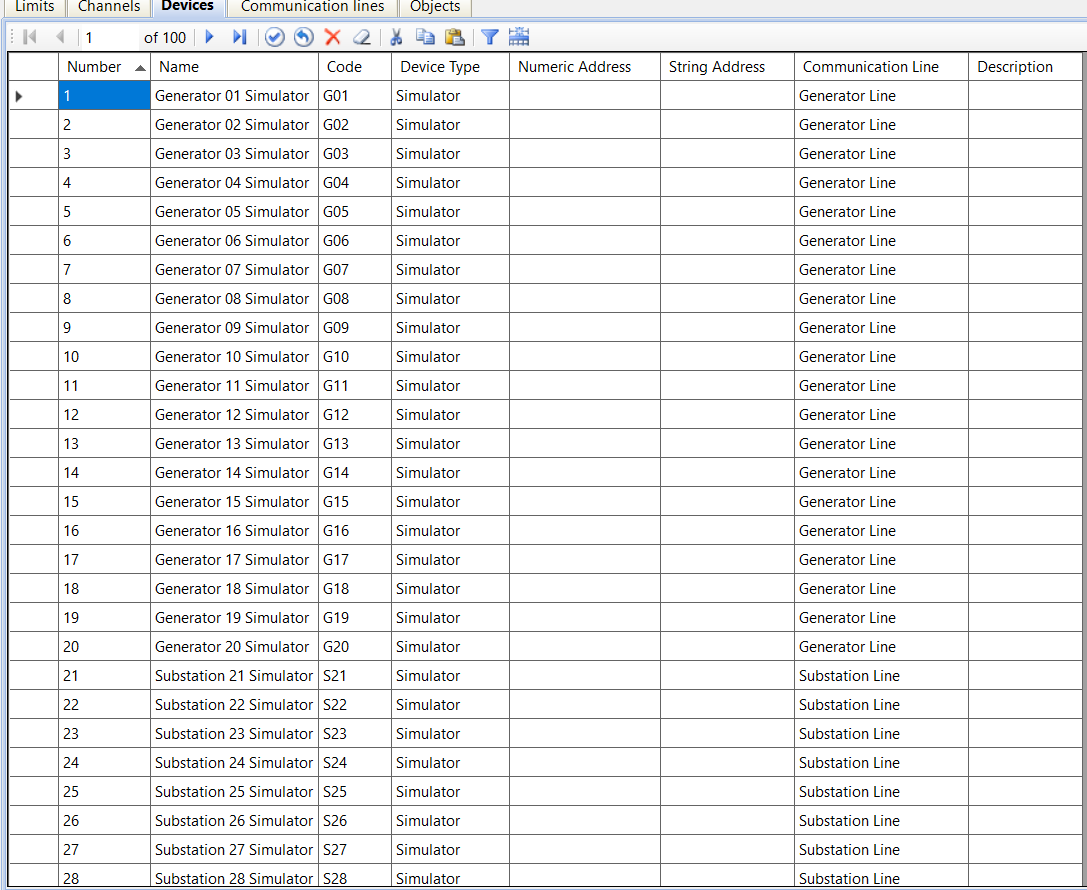
\includegraphics[width=0.95\textwidth]{live_agent_trace.png}}
\caption{Live agent trace showing the real-time telemetry readings and anomaly detection output for a selected agent during SCADA live operation.}
\label{fig:live_trace_1}
\end{figure}

\begin{figure}[H]
\centering
\fbox{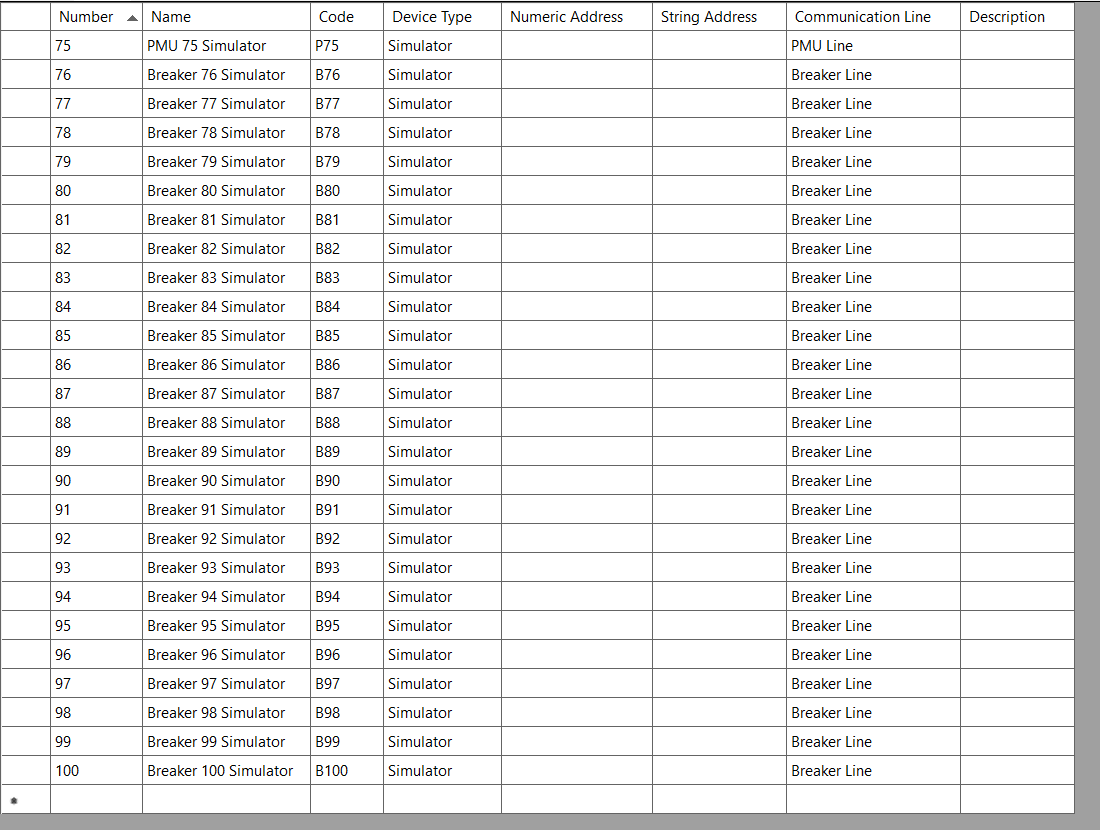
\includegraphics[width=0.95\textwidth]{live_agent_trace1.png}}
\caption{Live agent trace (continued) showing deviation scoring and risk assessment updates during active monitoring.}
\label{fig:live_trace_2}
\end{figure}

\begin{figure}[H]
\centering
\fbox{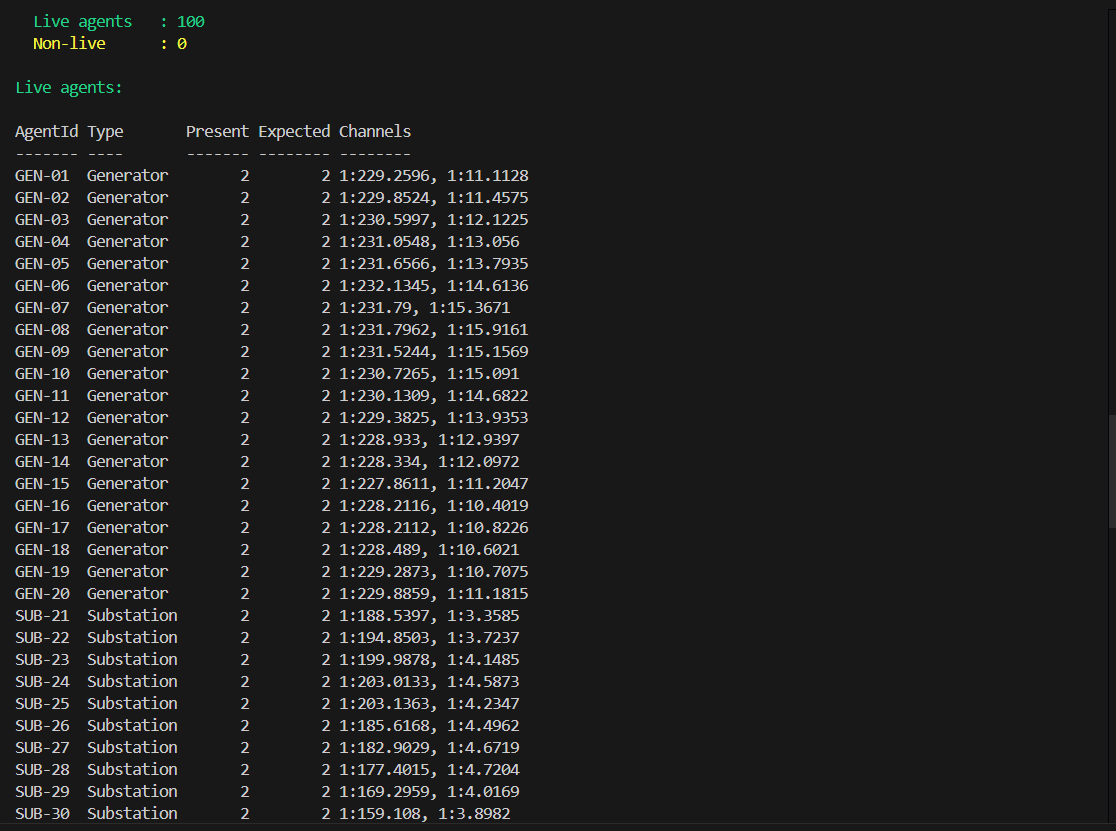
\includegraphics[width=0.95\textwidth]{live_agent_trace2.png}}
\caption{Live agent trace (continued) showing audit scheduling decisions and escalation actions in response to detected anomalies.}
\label{fig:live_trace_3}
\end{figure}


\subsection{Reconciling the Two Reported FPR Values}

This chapter reports two false positive rates for the same system, which can look contradictory at first glance. The 6.18\% figure cited in the primary thesis profile is the system level FPR with the audit protection window active (window=24 or window=288, both equivalent within a 24 hour cycle), and counts a false positive as an agent flagged as anomalous at a step where neither an attack nor a fault was actually applied after the mitigation pipeline has acted. The 18.0\% figure cited in the per attack analysis and Table~\ref{tab:three_modes} is the detector level FPR in eval mode (window=0), where the mitigation pipeline is intentionally bypassed so that every injected attack reaches the detector and the per attack TPR can be measured cleanly. The two numbers describe different operating points of the same software. The detector level FPR is the right number to cite when the question is about the raw detection algorithm, and the system level FPR is the right number to cite when the question is about end to end operational behaviour with auditing enabled.

\par \vspace{0.35cm}

\subsection{Limitations and Threats to Validity}

The evaluation in this chapter rests on four assumptions whose limitations are recorded here so that the reported numbers can be interpreted correctly.

\begin{enumerate}
    \item \textbf{Synthetic telemetry.} All experiments use the simulation grid and Rapid SCADA calculated channels rather than physical generators, breakers, PMUs or substations. The attack and fault perturbations injected in \texttt{grid\_env.step()} are parameter driven and do not capture every behaviour that real hardware would exhibit, particularly under sensor saturation, partial reporting or vendor specific deviations.
    \item \textbf{MITM remains the weakest class.} The five seed average TPR for MITM is between 72.3\% and 73.0\% across the three system sizes, while the other classes are at or above 78\%. MITM is the only class that mixes physical and cyber perturbations with smaller magnitudes than DoS, and its detector relies on a baseline aware jump z score that is sensitive to the seed dependent noise pattern. Further work on the MITM detector or a learnt classifier head for this class would be the most direct route to closing this gap.
    \item \textbf{Single 24 hour cycle.} Each evaluation run spans 288 timesteps, which corresponds to a single 24 hour grid cycle. Because the simulation length matches the longest audit protection window evaluated (window=288), the 2 hour and 24 hour protection windows produce indistinguishable results in this study. A multi day continuous operation experiment would be needed to separate them.
    \item \textbf{Single machine evaluation.} The latency numbers reported in Table~\ref{tab:latency} were measured on a single workstation with one CPU. The latency growth from $N=100$ to $N=500$ is consistent with linear batch size scaling on the LSTM inference path. Distributed inference or model quantisation would be required for $N$ much greater than 500.
\end{enumerate}

\par \vspace{0.35cm}

\subsection{Computational Cost of Layer C-4}

The fault signature detector added in this revision is a pure NumPy function evaluated on three physical features and four cyber features per agent per timestep. It does not invoke the LSTM, does not maintain learnt state, and does not iterate over history beyond the most recent observation. Its per agent runtime is dominated by three z score computations and a small number of conditional checks, and contributes negligibly to the end to end latency numbers reported in Table~\ref{tab:latency}. No latency regression was observed between the pre Layer C-4 sweep and the post Layer C-4 sweep at any of the three system sizes.

\par \vspace{0.35cm}

\subsection{Reproducibility}

All numbers in this chapter were produced by the code in this thesis project. Each summary table cites the exact seed range (42, 43, 44, 45, 46), the exact set of system sizes (100, 200, 500 agents), and the exact audit protection window used (0, 24 or 288 timesteps). The configurations were selected by setting the environment variables \texttt{SMARTGRID\_SEEDS}, \texttt{SMARTGRID\_SWEEP} and \texttt{SMARTGRID\_AUDIT\_PROTECTION\_WINDOW} before invoking \texttt{python -m smartgrid\_mas.run\_all}. The per run outputs (\texttt{summary.json}, \texttt{events.csv} and \texttt{audit\_events.csv}) are written to a path controlled by \texttt{SMARTGRID\_LOGS\_DIR}, which allows the eval mode and the two protected modes to be kept in separate directories for direct comparison.

\par \vspace{0.35cm}

\subsection{Overall Findings}

Based on the experimental evaluation presented in this chapter, the following key findings stand out:

\begin{enumerate}
    \item \textbf{The detector achieves strong per attack typing.} In eval mode the per attack true positive rates are 99.0\% for FDI, between 79\% and 83\% for DoS, between 72.3\% and 73.0\% for MITM, and between 98.4\% and 98.7\% for the new FAULT class, averaged over five seeds and three system sizes. These numbers show that the multi-layer architecture identifies the specific attack category, not just the presence of an anomaly.

    \item \textbf{The N=100 profile improves on the base paper in coverage and efficiency.} Risk mitigation (93.66\% vs.\ 87.9\%), cost efficiency (57.28\% vs.\ 42.5\%), and audit coverage (100\% vs.\ 93.8\%) all exceed the base paper, and the system adds per attack typing, live SCADA integration, and explainability. Detection accuracy (93.85\%) and system level false positive rate (6.18\%) reflect a high recall operating point (98.24\%) rather than a tuned best case.

    \item \textbf{Weighted ensemble fusion balances sensitivity and specificity.} The deviation weight of 0.48 combined with the LSTM probability weight of 0.52 produces a composite score that avoids both the over-sensitivity of deviation-only detection and the excessive conservatism of LSTM-only detection.

    \item \textbf{Hybrid scheduling improves cost efficiency over Q-learning alone.} The combination of Q-learning for discrete escalation decisions with gradient-based continuous optimisation achieves 57.28\% cost efficiency at N=100, exceeding the base paper's Q-learning-only 42.5\%.

    \item \textbf{Detection scales cleanly while the audit budget is the limiting resource.} Detection accuracy stays within a fifth of a percentage point of 93.7\% and the false positive rate stays near 6.3\% from N=100 to N=500. Audit coverage holds at 100\% to N=200 and drops to 91.44\% at N=500, and end-to-end latency increases from 55.04~ms to 254.69~ms, indicating that larger deployments need attention to the audit budget and inference batching rather than to the detection logic.

    \item \textbf{The new fault detector closes the largest per type gap.} Adding the Layer C-4 signature detector raised the FAULT class true positive rate from 8.1\% to 98.6\% at N=200 without reducing the FDI rate, and the cross-layer corroboration gate raised the MITM rate from 45.4\% to 71.1\% by removing noise driven false positives.

    \item \textbf{Live SCADA integration is operational but uses calculated channels.} The Rapid SCADA integration validates the full data pipeline from telemetry acquisition through detection and visualisation, while transparently acknowledging that the current deployment uses calculated channels rather than physical field devices.

    \item \textbf{The system works as a strong operational prototype.} Multi-layer detection, hybrid audit scheduling, SCADA integration, explainability, and full dashboard functionality together show that the framework is ready for deployment in controlled environments, with a clear path to physical device integration in future work.
\end{enumerate}
